\documentclass[12pt]{article}%
\usepackage{amsfonts}
\usepackage{fancyhdr}
\usepackage{comment}
\usepackage[a4paper, top=2.5cm, bottom=2.5cm, left=2.2cm, right=2.2cm]%
{geometry}
\usepackage{times}
\usepackage{amsmath}
\usepackage{changepage}
\usepackage{stfloats}
\usepackage{amssymb}
\usepackage{graphicx}
\usepackage{indentfirst}
\setlength{\parindent}{2em}
\setcounter{MaxMatrixCols}{30}
\newtheorem{theorem}{Theorem}
\newtheorem{acknowledgement}[theorem]{Acknowledgement}
\newtheorem{algorithm}[theorem]{Algorithm}
\newtheorem{axiom}{Axiom}
\newtheorem{case}[theorem]{Case}
\newtheorem{claim}[theorem]{Claim}
\newtheorem{conclusion}[theorem]{Conclusion}
\newtheorem{condition}[theorem]{Condition}
\newtheorem{conjecture}[theorem]{Conjecture}
\newtheorem{corollary}[theorem]{Corollary}
\newtheorem{criterion}[theorem]{Criterion}
\newtheorem{definition}[theorem]{Definition}
\newtheorem{example}[theorem]{Example}
\newtheorem{exercise}[theorem]{Exercise}
\newtheorem{lemma}[theorem]{Lemma}
\newtheorem{notation}[theorem]{Notation}
\newtheorem{problem}[theorem]{Problem}
\newtheorem{proposition}[theorem]{Proposition}
\newtheorem{remark}[theorem]{Remark}
\newtheorem{solution}[theorem]{Solution}
\newtheorem{summary}[theorem]{Summary}
\newenvironment{proof}[1][Proof]{\textbf{#1.} }{\ \rule{0.5em}{0.5em}}

\usepackage{mathtools}

\newcommand{\Q}{\mathbb{Q}}
\newcommand{\R}{\mathbb{R}}
\newcommand{\C}{\mathbb{C}}
\newcommand{\Z}{\mathbb{Z}}

\begin{document}

\title{STAT3003 Problem Sheet 3}
\author{ZHENG Weijia (William, 1155124322)}
\date{April 11, 2021}
\maketitle


\section{Q1}
\begin{figure}[htp]
    \centering % 图片居中
    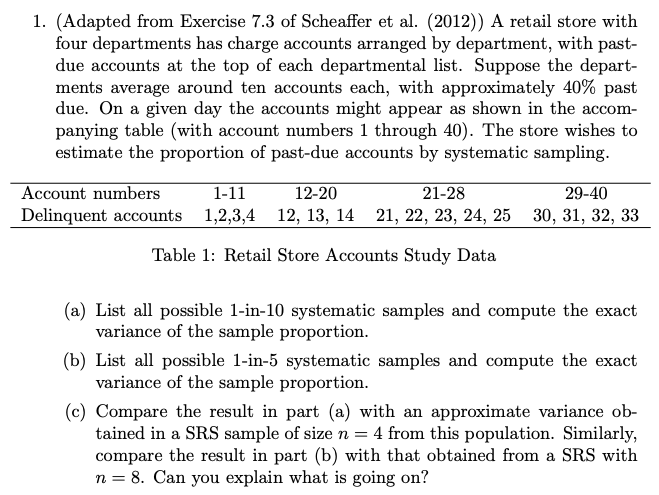
\includegraphics[width = 15cm]{img/Q1.png}
    %\caption{Section 6.1 Q8}
    %\label{fig:figure1label}
\end{figure}

\subsection{(a)}
We need to fix the starting point, when start at 1: the number of deliquent accounts is 3, 
the sample proportion is $\frac{3}{4}.$ 

When start at 2: the number of deliquent accounts is 4. The sample proportion is $1.$

When start at 3: the number of deliquent accounts is 4. The sample proportion is $1.$ 

When start at 4: the number of deliquent accounts is 3. The sample proportion is $\frac{3}{4}.$ 

When start at 5: the number of deliquent accounts is 1. The sample proportion is $\frac{1}{4}.$ 

When start at 6: the number of deliquent accounts is 0. The sample proportion is $0.$ 

When start at 7: the number of deliquent accounts is 0. The sample proportion is $0.$ 

When start at 8: the number of deliquent accounts is 0. The sample proportion is $0.$ 

When start at 9: the number of deliquent accounts is 0. The sample proportion is $0.$ 

When start at 10: the number of deliquent accounts is 1. The sample proportion is $\frac{1}{4}.$ 

Therefore the exact variance of sample proportion is $0.165.$

\subsection{(b)}
When start at 1: the number of deliquent accounts is 3. The sample proportion is $0.375.$

When start at 2: the number of deliquent accounts is 4. The sample proportion is $0.5.$

When start at 3: the number of deliquent accounts is 4. The sample proportion is $0.5.$

When start at 4: the number of deliquent accounts is 3. The sample proportion is $0.375.$

When start at 5: the number of deliquent accounts is 2. The sample proportion is $0.25.$

Hence the exact variance of sample proportion is $8.75\times 10^{-3}.$

\subsection{(c)}
Using the formulae $$Var(\hat{p})=\frac{N-n}{N-1}p(1-p).$$

And we have $p=0.4, N=40,$ therefore $Var(\hat{p})=0.0554.$

For $n=8$, $Var(\hat{p})=0.0246.$

When n=4, SRS's variance is smaller and when n=8, SRS's is larger.




\end{document}
